\section{Software}
%\subsection{Description}
The software of this project contains 3 parts:
\begin{itemize}
\item{The operating system configuration and modification to be fully compatible with the hardware used.}
\item{The website that is used by the young users to send pictures and messages to the old users.}
\item{The Vesta tab software that is used on the tablet to display the differents messages and pictures received by the old users.
}
\end{itemize}

\begin{figure}[!htb]
    \centering
    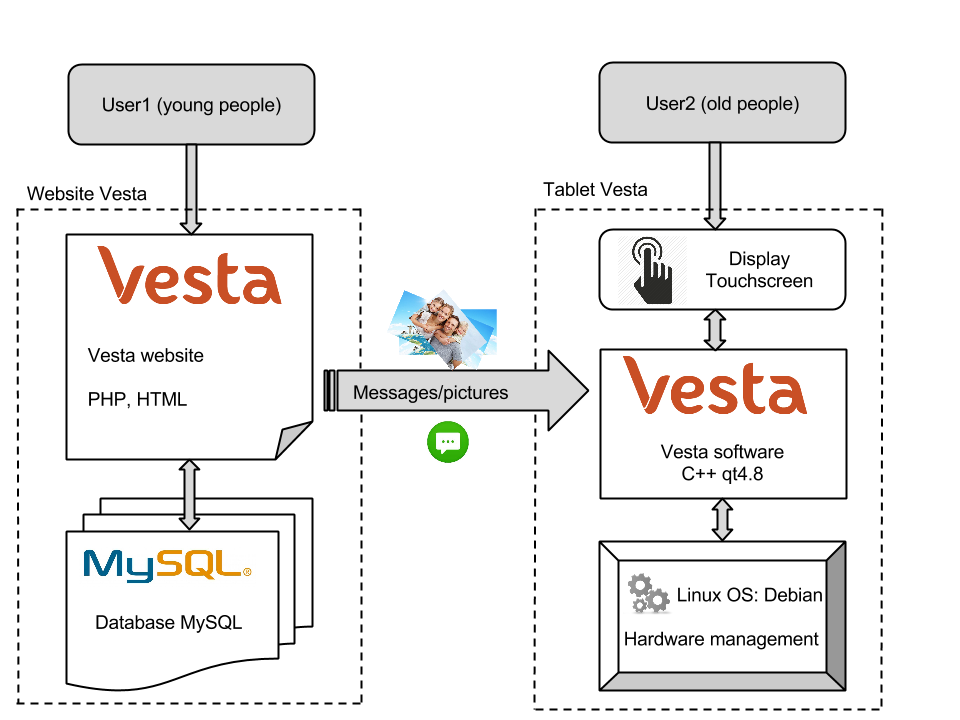
\includegraphics[width=0.9\textwidth,keepaspectratio]{chap/softFig/block_diagram_vesta2.png}
    \caption{Basic user flow.}
    \label{fig:user flow}
\end{figure}

\subsection{Operating system}
The OS used for this project is a debian. Debian is a linux distribution and was given by the conceptors of the beaglebone black.
\subsubsection{Drivers}
A lot of work on this linux distribution was made to be fully compatible with the chosen hardware.
The touch screen driver ed ft had problems with the original ? kernel of the distribution we used. The driver was not loading correctly from the device tree overlay. An upgrade to the ? kernel resolved the problem.
Then the scale of the touchscreen was not correct. 
When a touch event was done on the ? down corner,
 the mouse pointer moved to the center of the screen. Some configuration scripts had to be modified for the ? graphical display server.
\subsubsection{Display}
The touch screen works with 24 bits parallel interface so the X11 configuration file had to be modified to works correctly. The LCD output was initialy configured in 16 bits parallel interface.
The hardware management in linux is called a device tree blob. It’s a script that is compiled and is loaded at the OS startup. In this file, the driver for the touch panel was declared and the interrupt pins was defined. The resolution and frequency of the display is also configured in this script. The wifi chip also needs to load drivers at startup and tell the OS to connect to internet via this chip and with the SDIO protocol.
The file is located in /boot/dtbs/3.14xx/ and is called vesta.dtb (compiled) and the source is called vesta.dts. The file uEnv.txt located in /boot/ also need to define which device tree blob(dtb) the OS has to load at startup.
\begin{figure}[!htb]
    \centering
    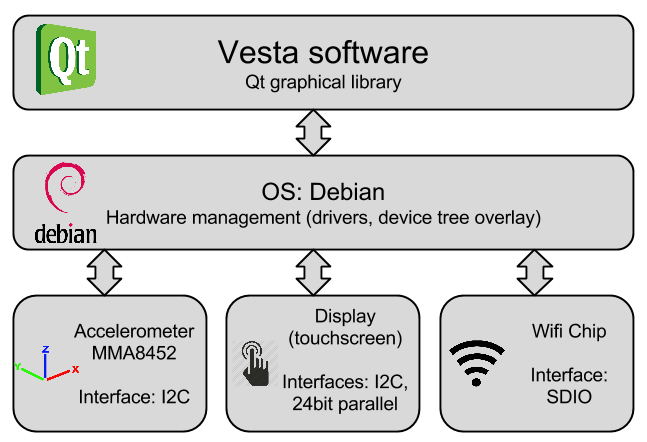
\includegraphics[width=0.9\textwidth,keepaspectratio]{chap/softFig/first_diagram2}
    \caption{Firmware dependencies.}
    \label{fig:firmware dependencies}
\end{figure}

\subsection{Website}
The website is used by the young users to send messages and pictures to the old user’s tablet.
The website contains a MySQL database, a php/html page that let the young user send a message and a php script used to parse the database to XML to be readable by the tablet.
\begin{figure}[!htb]
    \centering
    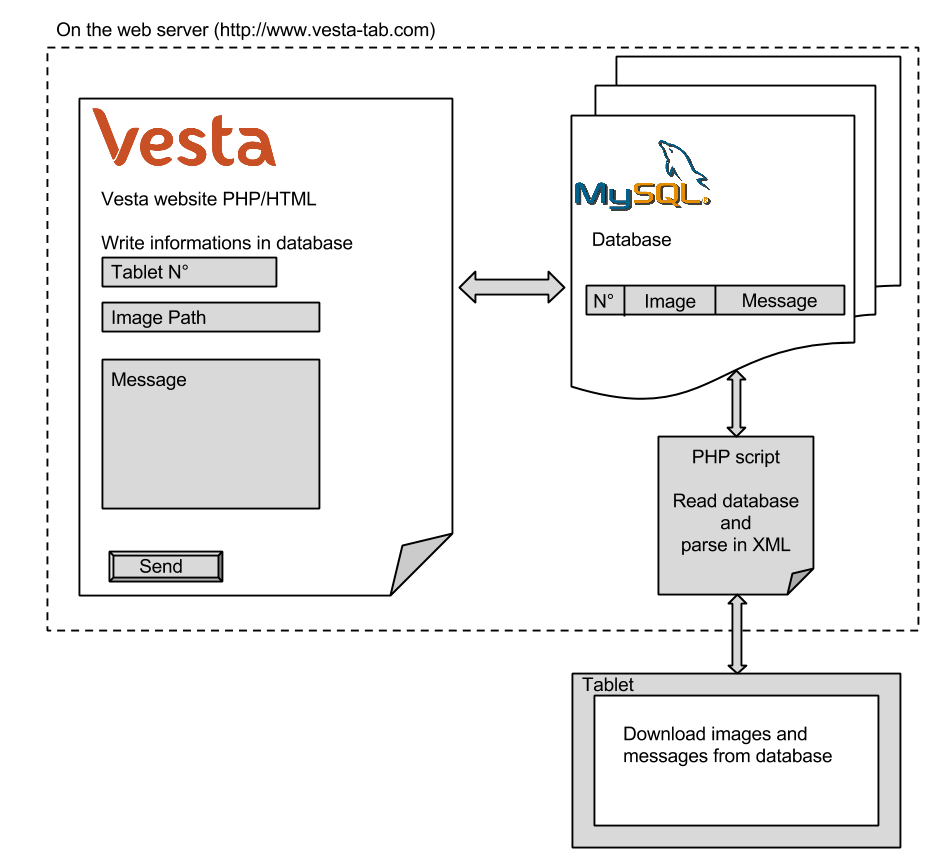
\includegraphics[width=0.9\textwidth,keepaspectratio]{chap/softFig/vesta_website2}
    \caption{Vest website architecture.}
    \label{fig:web archi}
\end{figure}

\subsection{Vesta software}
The Vesta software is used by the old users to receive and display the messages and pictures sent by the young users.
The software is made in C++ with Qt4.8/Qt quick 1.0. Qt is a free library used mainly to design softwares with graphical user interfaces (GUI). It is cross platform so with the same code it is possible to compile for linux,windows and mac.
The library contains also a lot of utils to facilitate the development of emmbedded interfaces and manages the touchscreen events like the swipes, clicks and more. A lot of documentation is available and a lot of users develop with it.
\begin{figure}[!htb]
    \centering
    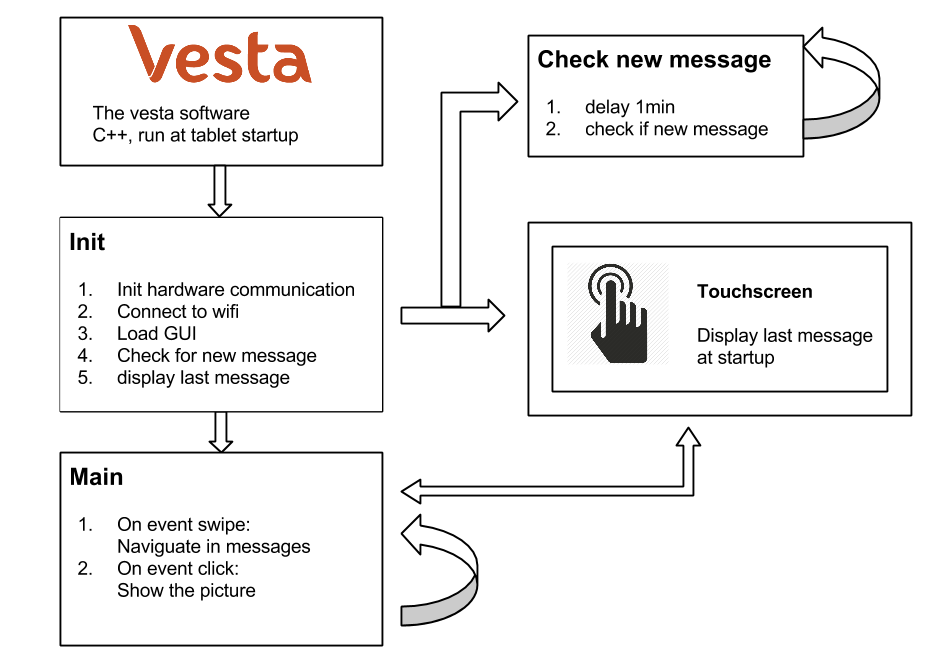
\includegraphics[width=0.9\textwidth,keepaspectratio]{chap/softFig/vesta_software_diagram2}
    \caption{Vesta software architecture.}
    \label{fig:soft archi}
\end{figure}